\subsection{Pipelining of Target Data Transfers}
\label{sub:pipelining}

Data transfers between host and device memory is a common bottleneck 
for heterogeneous applications. A basic optimization overlaps computation
with those data transfers. Further, devices often have limited memory 
capacities, which leads to optimizations that divide the computation
into pieces and stage in the data of upcoming pieces and stage out the
data of preceding ones while the current piece is executed. While this
\emph{pipelining} of data transfer and computation is a well understood
optimization, manual transformation to implement it involve many complex
and error-prone source code changes. 

We are developing interfaces that associate data transfers with loop iteration 
spaces and, thus, support automated pipelining. Figure~\ref{fig:pipeline} shows
an example that pipelines a stencil computation. The \texttt{map} clauses use 
the distributed loop's iteration variable to indicate that the compiler 
can divide the arrays along their first dimension and that three elements 
along that dimension of the input array are required to compute each element 
along that dimension of the output array. Thus, the compiler can transform 
the loop to perform chunks of the computation while pipelining the data.

\begin{figure}
\begin{minted}{c}
void func(double * A, double * An,
          int nx, int ny, int nz) {
#pragma omp target teams distribute    \
  pipeline(static)                     \
  map(pipeline,to:A[k-1:3][0:ny][0:nx])\
  map(pipeline,from:An[k:1][0:ny][0:nx])
  for(k=1;k<nz;k++) {
    #pragma omp parallel for
    for(i=1;i<nx;i++) {
      for(j=1;j<ny;j++) {
        An[Index3D (i, j, k)] =
        (A[Index3D (i, j, k + 1)] +
         A[Index3D (i, j, k - 1)] +
         A[Index3D (i, j + 1, k)] +
         A[Index3D (i, j - 1, k)] +
         A[Index3D (i + 1, j, k)] +
         A[Index3D (i - 1, j, k)])* c1
       - A[Index3D (i, j, k)] * c0;
      }
    } 
  }
}
\end{minted}
\caption{Pipelining Example\label{fig:pipeline}}
\end{figure}

Figure~\ref{fig:pipeline-perf} compares a prototype of this interface to a 
naive version that does not pipeline the loop~\cite{cui2017directive}. We 
present two pipelining strategies. Pipelined uses a buffer of the same size 
and layout as the naive version so it does not save memory space but splits 
the computation to overlap transfers. Pipelined-buffer uses smaller buffers
and transforms the accesses in the loop to decrease the memory capacity that
is required. In some cases, particularly the 3dconv and stencil kernels, the 
buffered version's greater locality actually improves performance. For the 
quantum chromo-dynamics kernel however it loses about 20\% performance 
compared to using the full amount of memory, but allows much larger 
problems to be run than otherwise fit on the device.

\begin{figure}
  \centering
  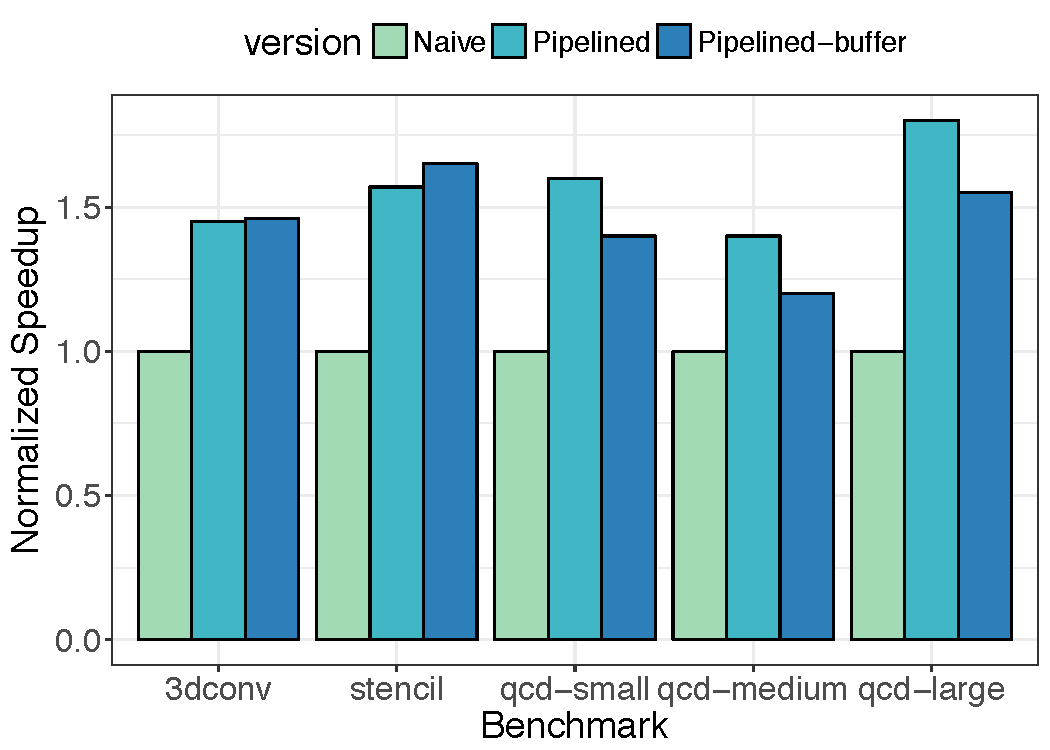
\includegraphics[width=0.5\textwidth]{pics/pipelining-perf}
  \caption{Pipelined Versus Buffered Data Transfers\label{fig:pipeline-perf}}
\end{figure}

